\let\textcircled=\pgftextcircled


\chapter{Literature Review}
\label{chap:lit_review}


\section{Components of a Self Driving Car}

Most self-driving cars consist of 4 main components: 
\begin{itemize}
	\item \textbf{LiDAR} - LiDAR provides highly detailed 3D information about the environment around the vehicle and objects in it. LiDAR operates by sending out pulses of lasers and recording the reflections of the pulses from objects. By comparing this with the time taken for the lasers to be reflected(time of flight) and their direction, the distance of these objects can be calculated and mapped in a point cloud. 
	\begin{equation*}
	distance = \frac{time \times \text{speed of light}}{2}
	\end{equation*}
	
	To achieve a high level of accuracy, a LiDAR unit has to send out a large enough number of lasers in different directions fast enough to create an accurate point cloud representation of the environment around it. To do so,  LiDAR units have multiple channels(emitter/receiver pairs) angled vertically that  emit hundreds of thousands of laser pulses  per second.
	
	LiDAR units require complex optical systems that are expensive to build. As a result,  they are the most expensive sensor in AVs with the top end such as Velodyne HDL-64E shown in figure \ref{fig:lidar} costing around 75,000\$. More channels allow for a more accurate representation of the surrounding environment which is necessary for safer navigation of AVs. However it is worth noting that the cost of LiDAR units increases proportionally with the number of channels. 
	As such, different companies have are exploring different design methods that are cheaper but still able to offer the same performance as the top end LiDAR units. 
	This has resulted in the development of different types of LiDAR units as shown below. 
	\begin{itemize}
		\item \textbf{Mechanical Mirror}
		\item \textbf{Solid State}
		\item \textbf{Optical Phase Array}
		\item \textbf{Microelectromechanical systems (MEMS)}
		\item \textbf{3D Flash}
	\end{itemize}

	 
	 \begin{figure}[h]
	 	\centering
	 	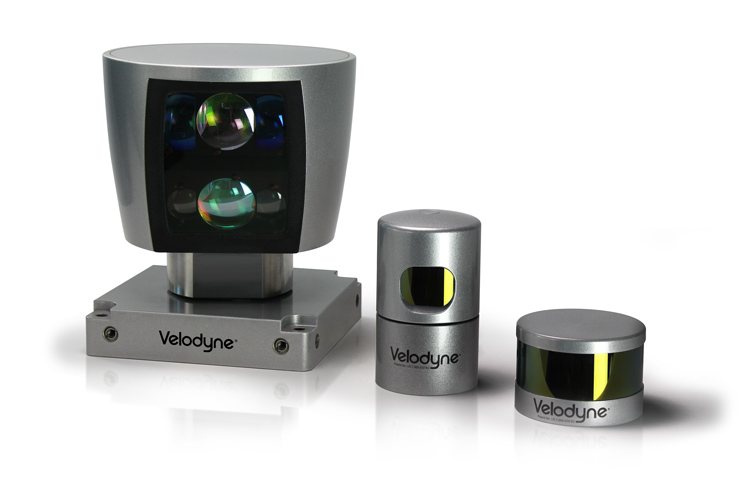
\includegraphics[width=\textwidth]{media/hdl-family.png}
	 	\caption{Velodyne LiDAR family. From left: Velodyne HDL-64E , HDL-32E , PUCK}
	 	\label{fig:lidar}
	 \end{figure}
	
	\item \textbf{Cameras} - Cameras mounted on the vehicle are used for classification and identification of various objects on the road. This is important for recognising traffic rules from traffic signs or road markings as well as determining the nature of objects on the road. 
	Cameras can also be used to create 3D maps of the surrounding environment.By combining two cameras, a stereo image can be captured that provides depth information. Alternatively, by combining a camera and IR Laser sensor for depth estimation, RGB-D \cite{henry2010rgb} images are obtained and mapped in a point cloud.
	
	\item \textbf{Position Estimators} - Position estimators are a group of sensors used for navigation of the vehicle. These include GPS systems, odometers and gryometers. 
	\item \textbf{Distance Sensors} - Distance sensors such as radars and sonars are important for gauging the distance of objects on the road. 
	Radars are the most commonly used distance sensors and they work by transmitting radio waves and recording the reflected radio waves from objects. As compared to cameras and LiDARs, radars work well in a variety of low visibility scenarios such as poor weather. 
	However, the reflectivity of these radio waves depends on the nature of objects, their size, absorbtion characteristics and the transmitting power. As such, it is may not be effective for detecting objects with low absorbtion characteristics such as pedestrians and animals.
	
	\item \textbf{Processing Unit} - In order to process all the data from the sensors in the vehicle, AVs require powerful processing units in order to be able to process all this data in real time. Most of the ML/AI algorithms used for detecting and identifying objects from LiDAR and camera data demand large amounts of processing power. This is achieved through the use of CPUs, GPUs, Field Programmable Gate Arrays(FPGA)\cite{brown2012field}, Application Specific Integrated Circuits(ASICs)\cite{smith1997application} or combinations with each other. 

\end{itemize}


\begin{figure}[t]
	\centering
	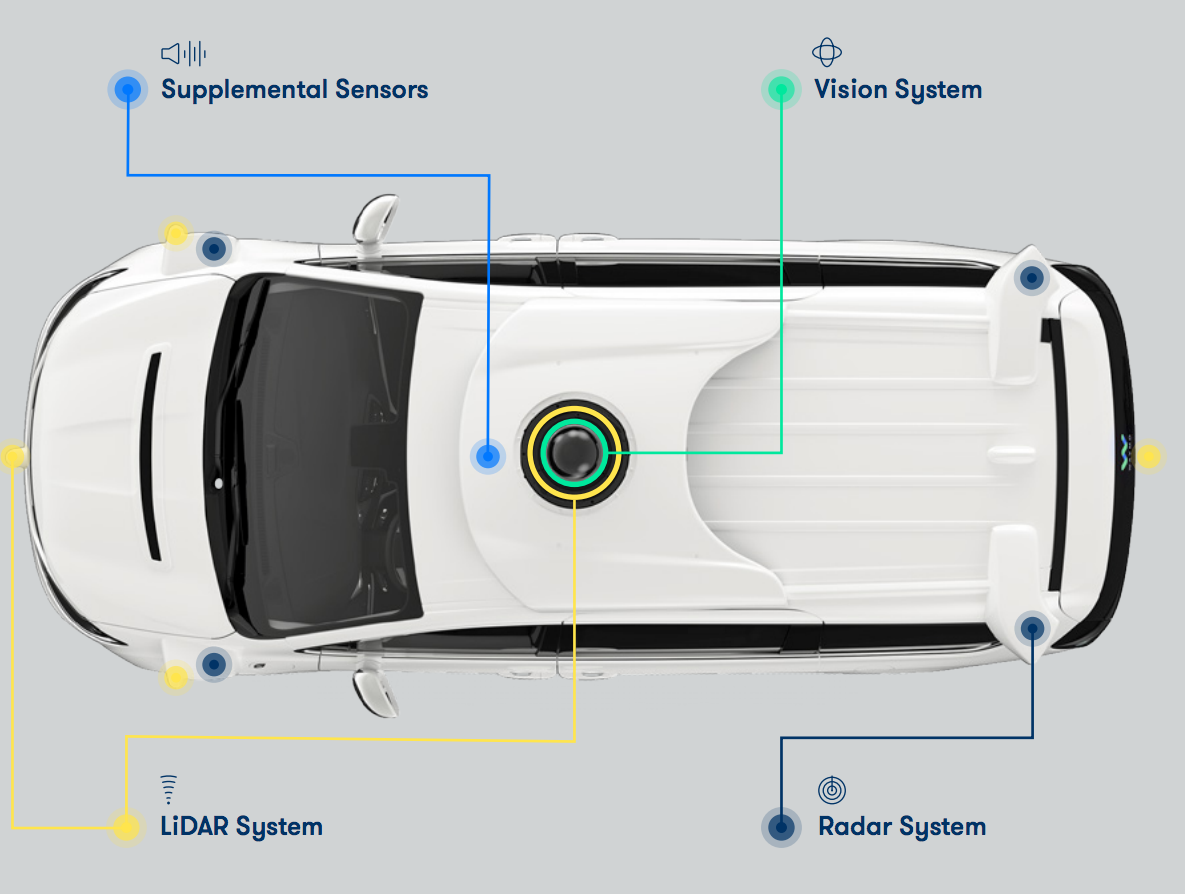
\includegraphics[width=\textwidth]{media/waymo.png}
	\caption{Components of Waymo's Self Driving Car \cite{waymo_2018}}
	\label{fig:my_label}
\end{figure}



\subsection{Legal, Ethical and Economic Considerations}

The classic ethical dilemma for self driving cars poses a scenario whereby AVs are presented with a situation whereby a fatal accident is inevitable. For example, the AV either has to crash into a group of people in order to save the life of a passenger or to crash itself and sacrifice the life of the passenger. This dilemma highlights important legal, ethical and economic considerations to be considered by companies involved in the production of AVs and their corresponding systems. 


According to \cite{gasser2016fundamental}, there are no public laws that cover the  use of independent autonomous vehicles in public spaces. In his article, he cites the fundamental issue as "understanding and accepting the effect of AVs as an independent action by a machine". Due to the lack of public laws on their use, he proposes extending fundamental rights such as the right to life into the framework for creating laws that cover emerging technologies that have an effect on the public, that are otherwise not accounted for in traditional laws. 

Bearing this in mind, it is important to note that despite improvements in traffic safety over the years, 94\% are still caused by human beings with a large majority of them being fatal with the current human error rate being 1 in 100 million miles. This creates a realistic baseline that can then be extended in evaluating the performance of AV systems. As such, if the risk of automation is lesser than the risk of human vehicle control then the AV would be beneficial. Consequently, the AVs are not to be considered as perfect systems.

With regard to economic considerations, car manufucturers involved in the production of AVs have to ensure that their AVs are able to handle numerous scenarios even if they are rare or considered statistically impossible. They should also be required to take legal liability in case any of their system components are defective and result in failures or accidents. This is important for customer trust without which they will not be able to convince customers to shift to AVs. In addition, for the adoption of AVs to be widespread, they have to be reasonably priced and efficient. With the current prices of the the various components and their power consumption, the adoption of AVs at the moment is not viable. 




AVs have three main modes of operation namely,
\begin{itemize}
	\item \textbf{Perception} - This is the first step which involves processing the input from the sensors. In this mode tasks such as object detection and tracking, lane detection, traffic sign detection and recognition are performed.
	\item \textbf{Planning} - This is the next step after detection and recognition tasks are performed . In this stage route and trajectory planning algorithms are run to to plan how the vehicle should navigate in the immediate environment as well as a route to a target location. These algorithms are required to handle complex situations to ensure safety of the passengers and other road users. 
	\item \textbf{Control} - This stage involves the execution of the plans created in the planning stage. This stage is crucial as the actuators involved in steering and movement have to be able to be able to accurately follow the plans. This involves calculation of energy and forces. At this stage the trajectories and movement of other road users and objects have to be calculated in order to anticipate and avoid any accidents. 
	
\end{itemize}



\section{Industrial Approaches}
In an effort to achieve the forementioned requirements, different companies have used different approaches in order to do so.
However, a few constraints have to be considered as outlined in \cite{lin2018architectural}
\begin{itemize}
	\item \textbf{Performance} \\
	At the moment there are no clear regulations as to how fast the perception, planning and control pipeline should be. However according to research by Brown et al. \cite{brown1994human}, humans take around 600 ms to respond and brake when expecting an interruption, however this figure shoots to 850 ms when an unexpected situation arises. In addition, Newell et al \cite{newell1985prospects}, established that the fastest human response time is between 100-150ms. These figures can be used as a baseline while developing a pipeline. In this pipeline, there are two factors to consider, namely the frame rate (frequency of the data from sensors) and the processing latency (time taken to process data). As such, an AV system should be able to react within 100ms, that is, faster than the human response time.
	
	\item \textbf{Storage} \\ 
	AVs should be able to store maps of different areas with fine granularity for accuracy during localisation. As a result, the storage of these maps can run into tens of Terabytes. Despite recent advances in cloud technology and the emergence of 5G connectivity that is significantly fast. Downloading these maps would take significant time and would also render the car unusable in case of no internet connectivity. As such, the vehicles should have enough storage to store these maps locally. 
	
	\item \textbf{Power} \\
	Most of the major industry players have moved to electric-vehicles for their AV systems. Depending on the equipment and sensor configurations used in these systems, the power usage can range from 500 watts to 1.5 kilowatts. Given that the AVs have limited battery capacity, heavy power consumption by these systems can lead to poor driving ranges hence making the cars less viable. As such the configuration of these systems has to be carefully considered to ensure a reasonable driving range. 

	\item \textbf{Thermal} \\
	Processing components in the AV systems such as CPUs and GPUs require a significant amount of energy to cool. This is to necessary to ensure that they operate within their recommended thermal operating range. Failure to do so could result in the failure of these systems. As such, additional cooling systems have to be installed in the vehicle in order to ensure this. 
	
\end{itemize}
Following the discussion above, the next subsections will review how different industry players are implementing their AV systems with special focus to the issue of perception
\subsection{Camera}
Mobileye, is one of the leading industry players in the development of AV. It was recently acquired by Intel and believes that AVs should be able to accurately and safely navigate using cameras only given the fact that humans are able to do so with vision only. Previously, MobilEye was a supplier of vision systems for Advanced Driver Assistance Systems and had a partnership with Tesla to supply their vision systems prior being acquired by Intel. 
Given their extensive background in developing these vision systems, the partnership with Intel aims to develop a complete autonomous driving package. Intel  in it's part has been developing an a
 

\subsection{Camera and  Radar}
A major industry player that is using the camera and radar configuration is Tesla. Elon Musk, the founder, believes that LiDAR is not necessary for AV perception. However, following a recent accident whereby a passenger was killed in a crash while the vehicle was on 'autopilot', his statement was critiqued as LiDAR could have detected the presence of the woman. As mentioned in the discussion of components, Radar does not perform particularly well with organic objects due to their low reflectivity. Furthermore, due to the fact that it was night time, the cameras had a low visibility range and therefore this system configuration was not robust enough. 


\subsection{LiDAR, Camera and Radar}
Waymo, GM Cruise and Uber all use a combination of LiDAR, camera and radar. This combination has proven to be robust and accurate.

 However, in order to process the amount of fused data, they require large amounts of processing power which in turn may lead to increased power usage. 

\subsection{Accelerator Architectures}
Accelerator architectures can be described as the systems responsible for processing the data from the sensor units. These systems are used to run ML/AI algorithms that are used for the perception, planning and control pipeline. 
\subsubsection{CPUs}
With the 



\subsubsection{GPUs}

GPUs are the most common 
CPUs, GPUs, FPGAs, ASICs all offer differe


\section{Related Research} 

Following the discussions in the previous sections it is clear that systems to be used in AV have to fulfill certain requirements, namely:
\begin{itemize}
	\item \textbf{Robust}
	\item \textbf{Reproducible}
	\item \textbf{Validatable}
	\item \textbf{Viable}
\end{itemize}

As the aim of the project is to develop an object detection region proposal network for LiDAR object detection, this section will review research in the area of point cloud object detection. These papers will be analysed against the list of requirements provided above. 

\subsection{Classic Computer Vision}
With regard to perception, classic computer vision methods have advanced over the years from simple algorithms such as SIFT\cite{lowe1999object} and SURF\cite{bay2006surf} which use descriptors to detect interesting point in images for object detection to much higher level representations such as the Histogram of Gradient(HOG)\cite{dalal2005histograms} or Haar Features\cite{viola2001rapid}  that were uses in classifiers.  However, these methods have been unreliably slow and not as accurate. In addition these features are only able to model 2D data and therefore when applied to 3D data such as point clouds they are unusable. In addition, these feature detectors have to be handcrafted manually which is a tedious process. As a result,  such classical methods can not be used in AVs as they do not fulfill any of the requirements above. 


\subsection{Deep Neural Networks}

The emergence and development of Deep Neural Networks such as Convolutional Neural Networks(CNNs)\cite{lawrence1997face} has offset the reliance of classical methods of object detection in images by allowing for features to be automatically learnt by the network without the need for manual feature extraction. This is due to the fact that these networks have numerous number of deep layers that are able to capture these features.  

\textbf{Monocular Vision}




\textbf{Stereo Vision}



\textbf{RGB-D}



\textbf{LiDAR/Camera}



\textbf{LiDAR}




Deep neural networks overcame the problem of having to handcraft features to be used in a classifier. Their ability to automatically learn features has been greatly influential
However, this has only been applicable to dense 2D data from cameras and not to sparse 3D data from LiDAR and RGB-D sensors that create cloud points. Cloud points are a geometric representation of unordered set of points. This representation is 3D in nature and as such contains important depth information that can be used to measure the size and shape of objects. Initial attempts to work with this data required hand crafted methods to first represent this information on a 2D plane before running the computer vision algorithms on these representations. 











\section{Deep Learning Framework}

A recurring theme that is central to the operation of AVs is object detection. Object detection is crucial for safe operation of AVs as it forms the first step before any planning and control. To achieve real-time results, deep learning techniques are being developed for this task. As mentioned in the previous chapter one of the main deliverables will be an end to end RPN model for detecting objects in point clouds. In order to develop this I will make use of a deep learning framework. 
At the moment, there are various distributions of deep learning frameworks that are available for different programming languages. 
A few popular ones include:
\begin{table}[H]
	\centering
	\begin{tabular}{|c|c|}
		\hline
		Framework & Programming Language(s)  \\ \hline
		Tensorflow &  Python, C++ , R  \\ \hline
		PyTorch & Python  \\ \hline
		Caffe & C, C++, Python, MATLAB \\ \hline
		MXNet & Python, C++, R, Julia \\ \hline
		Microsoft Cognitive Toolkit/CNTK & Python, C++ \\ \hline
		
	\end{tabular}
	\caption{Popular deep learning frameworks}
	\label{table:dlframeworks}
\end{table}

I intend to use Tensorflow on Python to implement the RPN. As a RPN is a form of CNN, the next sub section will detail the process of developing a CNN on TensorFlow. 

\subsection{TensorFlow CNN}
\begin{figure}
	\centering
	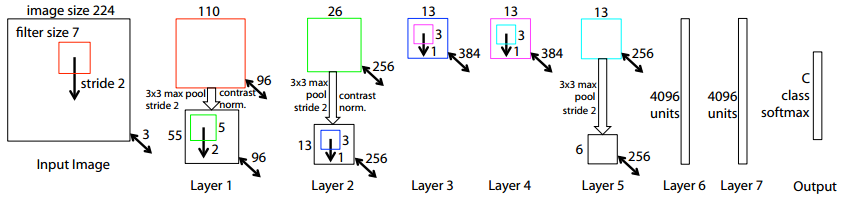
\includegraphics[width=\textwidth]{media/cnn.png}
	\caption{CNN Visualisation \cite{zeiler2014visualizing}}
	\label{ fig:cnn_vis}
\end{figure}

\begin{lstlisting}[language=Python, caption=Simple CNN  implementation using Tensorflow in Python \cite{abadi2016tensorflow}]
	def cnn_model_fn(features, labels, mode):
	"""Model function for CNN."""
	# Input Layer
	input_layer = tf.reshape(features["x"], [-1, 28, 28, 1])
	
	# Convolutional Layer #1
	conv1 = tf.layers.conv2d(
	inputs=input_layer,
	filters=32,
	kernel_size=[5, 5],
	padding="same",
	activation=tf.nn.relu)
	
	# Pooling Layer #1
	pool1 = tf.layers.max_pooling2d(inputs=conv1, pool_size=[2, 2], strides=2)
	
	# Convolutional Layer #2 and Pooling Layer #2
	conv2 = tf.layers.conv2d(
	inputs=pool1,
	filters=64,
	kernel_size=[5, 5],
	padding="same",
	activation=tf.nn.relu)
	pool2 = tf.layers.max_pooling2d(inputs=conv2, pool_size=[2, 2], strides=2)
	
	# Dense Layer
	pool2_flat = tf.reshape(pool2, [-1, 7 * 7 * 64])
	dense = tf.layers.dense(inputs=pool2_flat, units=1024, activation=tf.nn.relu)
	dropout = tf.layers.dropout(
	inputs=dense, rate=0.4, training=mode == tf.estimator.ModeKeys.TRAIN)
	
	# Logits Layer
	logits = tf.layers.dense(inputs=dropout, units=10)
	
	predictions = {
	# Generate predictions (for PREDICT and EVAL mode)
	"classes": tf.argmax(input=logits, axis=1),
	# Add `softmax_tensor` to the graph. It is used for PREDICT and by the
	# `logging_hook`.
	"probabilities": tf.nn.softmax(logits, name="softmax_tensor")
	}
	
	if mode == tf.estimator.ModeKeys.PREDICT:
	return tf.estimator.EstimatorSpec(mode=mode, predictions=predictions)
	
	# Calculate Loss (for both TRAIN and EVAL modes)
	loss = tf.losses.sparse_softmax_cross_entropy(labels=labels, logits=logits)
	
	# Configure the Training Op (for TRAIN mode)
	if mode == tf.estimator.ModeKeys.TRAIN:
	optimizer = tf.train.GradientDescentOptimizer(learning_rate=0.001)
	train_op = optimizer.minimize(
	loss=loss,
	global_step=tf.train.get_global_step())
	return tf.estimator.EstimatorSpec(mode=mode, loss=loss, train_op=train_op)
	
	# Add evaluation metrics (for EVAL mode)
	eval_metric_ops = {
	"accuracy": tf.metrics.accuracy(
	labels=labels, predictions=predictions["classes"])}
	return tf.estimator.EstimatorSpec(
	mode=mode, loss=loss, eval_metric_ops=eval_metric_ops)

\end{lstlisting}

\begin{enumerate}
	\item Convolution layer 
	\item Pooling Layer
	\item  Dense Layer 
	\item  
	\item 
\end{enumerate}




